\section{Theory}
The contents of this chapter are, if not otherwise specified, derived from the guide to the experiment \cite{anleitung}
\subsection{Spin and nuclear spin}
The spin or intrinsic angular momentum of a elementary particle is an intrinsic property of particles from the family of the fermions. Members of this family, such as protons, neutrons and electrons all have a spin of $s=\frac{1}{2}$.
The spin can be explained semi classically, as rotation of the particle around its own 'centre of mass', with fixed frequency and variable axis of rotation. 
However, this illustration only makes sense in finite-size particles, of course. Just as with the angular momentum, not all three spin components can be defined at the same time, but only the amount and projection on a freely selectable 'quantization axis'.
The possible spin quantum numbers are $$ \left|\vec{S}\right| = \hbar \sqrt{S\left(S+1\right)}$$ with $S = 0, \frac{1}{2}, 1, ...$ and Planck's constant $\hbar$. 
Atomic nuclei are also assigned a spin, the nuclear spin, which is defined with the nuclear spin number $I$, analogue to the spin: 
$$\left|\vec{I}\right| = \hbar \sqrt{I\left(I+1\right)}$$
The nuclear spin number is also quantified in its direction. Analogue to the electron spin, the projection of the nuclear spin can also assume certain states as , e.g. with the z-axis as the quantization axis $I_z = m_I \hbar$ with $-I\le m_I \le + I$. In total there would be  $2I+1$ different states for $I_z$. Protons or the nucleus of $^{19}$F both have a nuclear spin number of $I=\frac{1}{2}$. So both have only two possible states: $m_I = \pm \frac{1}{2}$. They can only align parallel or antiparallel with the quantization axis in the experiment.

\subsection{Magnetic momentum}
The spin of a quantum mechanical particle is connected to a magnetic dipole momentum $\vec{\mu}$, the ratio of both is described as the gyromagnetic ratio $\gamma$.
$$\vec{\mu}=\gamma\vec{I}\qquad \textrm{with}\quad \gamma = \frac{g_I\mu_K}{\hbar}$$
The constant $g_I$ is the nuclear g factor, which is to be calculated during the exam. $g_I$ has no dimension and is unique for each nucleus. The second constant $\mu_K$ is the nuclear magneton, which is computed analogue to the Bohr magneton:
$$\mu_K = \frac{e\hbar}{2m_p}$$
The difference between those two is that for the Bohr magneton the elecron mass is used and for the nuclear magneton the proton mass. 
In the ground state of atomic nuclei, the nucleons are arranged according to the Pauli principle so that each orbital is occupied by two protons or neutrons of opposite spins. If now a eu-nucleus (with an even number of protons and an uneven number of neutrons) or if an ue-nucleus (where the even and uneven nucleons are reversed) is present, an unpaired nucleon remains. This leads to an half-digit total spin. For a uu-nucleus two unpaired nucleons remain resulting in an integer total spin. In a ee-nucleus all nucleons are paired, therefore the total spin is zero. Examples for ee-nuclei are $^{16}_{8}$O and $^{12}_6$C. Therefore it is possible to measure the spin of hydrogen $I=\frac{1}{2}$ utilizing glycol (C$_2$H$_6$O$_2$) and water (H$_2$O) samples. For the $^{9}_{19}$F nucleus with 9 protons and 10 neutrons the total spin is also $I=\frac{1}{2}$.
\subsection{Interaction with magnetic fields and radiation (nuclear magnetic resonance)}
Classically the the energy of a magnetic dipole moment $\hat{\mu}$ in a magnetic field $B$ is described by the equation \ref{eqDipol}.
\begin{equation}
E=-\hat{\mu}\cdot B
\label{eqDipol}
\end{equation}
If the magnetic field goes in the z direction this can be written in quantum mechanics like in equation \ref{Zeeman} and is called Zeeman-splitting. 
\begin{equation}
E = - \mu_K g_I m_I B_x
\label{Zeeman}
\end{equation}
Here the energy niveaus are degenerated if there is no outer magnetic field, with the magnetic field the levels spits up depending on the quantum number $m_j$. In figure \ref{ZeemanBild} we see this splitting up under the influence of the magnetic field. 
\begin{figure}[h]
	\begin{tikzpicture}
	\draw (1,0) -- node[above] {$I=1$} (3,0);
	%\draw (3.2,0) -- (4,0);
	%\draw (3.2,0.1) -- (4,1);
	%\draw (3.2,-0.1) -- (4,-1);
	\draw (4.1,0) -- (6,0) node[right] {\quad$0$} ;
	\draw (4.1,1) -- (6,1) node[right] {\quad$1$} ;
	\draw (4.1,-1) -- (6,-1) node[right] {\quad$-1$} ;
	\node at (2,2) {$B=0$};
	\node at (5,2) {$B>0$}; 
	\node at (6.6,2) {$m_j$};
	\end{tikzpicture}
	\centering
	\caption[Zeeman Splitting]{Zeeman splitting for $I=1$}
	\label{ZeemanBild}
\end{figure}\\
The difference energy $\Delta E$ between attached $m_j$ can be written as follows:
\begin{equation}
\Delta E = g_I \mu_K B
\end{equation}   
This amount of energy needs to be absorbed or emitted for the spin to change its direction. This can happen through photons or by interaction with a 'Strahlungsfeld'. Since a certain amount of energy is needed it happens only at certain frequencies. This so called resonance frequency is given by:
\begin{equation}
	\nu = \frac{\Delta E}{h}=\frac{g_I\mu_KB}{h}=\frac{\gamma B}{2\pi}	
\end{equation}
If a spin absorbs energy of the 'Strahlungsfeld' and changes into a higher level the intensity of 'Strahlungsfeld' decreases which is measurable. 
\section{Relaxation Effects}
In thermal equilibrium the occupation number are Boltzmann distributed.
The probability of a state depending on energy and temperature is given through:
\begin{equation}
p_i=\frac{e^{\nicefrac{-E_i}{kT}}}{Z}
\label{Boltzmann}
\end{equation}
Here k is the Boltzmann constant and Z is the canonical partition function of all the states in the system. The probability $p_i$ can also be given by: $$p_i=\frac{N_i}{N}$$ With that the relationship between two states $1$ and $2$ is given through eq.\ref{Boltzmann2}
\begin{equation}
\frac{N_1}{N_2}=e^{-\frac{E_1-E_2}{kT}}=e^{-\frac{\Delta E}{kT}}
\label{Boltzmann2}
\end{equation}
That means that there will always be more particles in the lower state than in an upper one. It follows as well, that the occupation numbers should equalize and with it the measurable effect. This is not happening because of so called relaxation effects. There are two major relaxation effects:
\begin{enumerate}
	\item Spin-Lattice Relaxation: Here the exited nucleus give their energy to the lattice structure of the molecule. This energy is lost to the 'Strahlungsfeld'.
	\item Spin-Spin Relaxation: One nucleus creates a magnetic field at the another nucleus which shifts the outer magnetic field increasing or decreasing it. This leads to an change in the width of the absorption line.
\end{enumerate} 
\section{Hall Sensor}
The Hall sensor is used to measure magnetic fields. It uses the Hall effect. The effect happens to electrons in a cable effected by a outer magnetic field. Here the electrons are pushed under the Lorenz force $\vec{F}_L=q\cdot(\vec{v}\times \vec{B})$ to the side of the cable till certain voltage is reached which counters the Lorenz force $F_L=F_E$. This voltage $U_{Hall}$ can be measured. Equation \ref{Hall} gives a relationship between the Hall voltage and the magnetic field.
\begin{equation}
U_{Hall}=H\frac{IB}{d}
\label{Hall}
\end{equation}
\begin{enumerate}
	\item[•] $H$: Is the Hall constant $\frac{1}{ne}$ with $n$ the electric charge density and $e$ the charge of an electron.
	\item[•] $I$: The current.
	\item[•] $B$: The magnetic field.
	\item[•] $d$: The width of the cable.
\end{enumerate}
\subsection{Lock-in Amplifier}
The lock-in method is used to make small signal visible inside of huge noise. To do this the main signal will be multiplied with a reference signal and integrated with a low pass filter and amplified.
\section{Method of Measuring}
\subsection{Measuring the Magnetic Field}
To measure the magnetic field the earlier discussed Hall sensor is used. It is put onto a long rod which a cm scale. That way it can be put into the magnetic field and measure it for certain depths.  When the magnetic field doesn't change while changing the position of the Hall sensor the field is homogeneously. 
\subsection{Measurement of the Resonance Frequency}
To measure the resonance frequency the constant field method is used. Here the 'Strahlungsfeld' of the NMR (Nuclear Magnetic Resonance) Oscillator is set at a constant frequency and the magnetic field is changed with a wave to check for the correct resonance frequency. If this frequency is hit the spins will change and the 'Strahlungsfeld will lose energy which can be seen in the change of the amplitude. For the magnetic field two electromagnets are used which have to smaller ones attached to vary the field with the help of a wave. To measure the correct frequency two different methods are used.
\subsubsection{Sine Modeling Method}
The first one uses a sine wave to change the magnetic field. That means that the correct frequency will be hit two times each sine period and with this two absorption lines. To find the exact resonance frequency the minima need to be equidistant, since at this point they will be at the 'Nulldurchgang' of the modulated magnetic field. At this point the correct frequency to the set magnetic field is found. The experimental setup for this part can be seen in figure \ref{Exp_part1}.
\begin{figure}[h]
	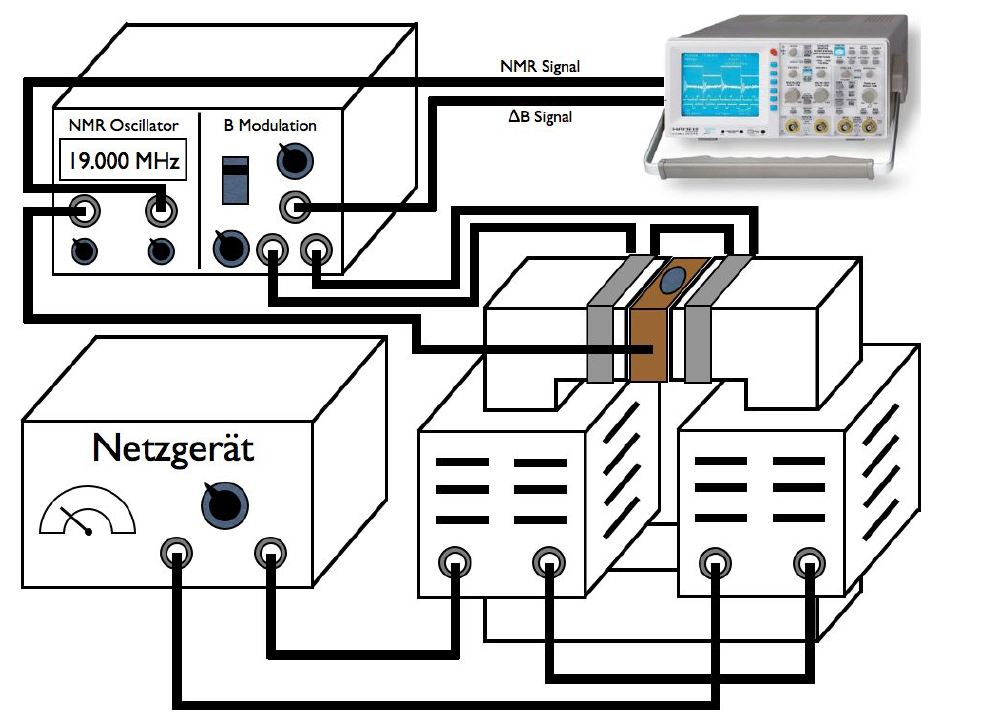
\includegraphics[scale=1]{Bild/Setup1}
	\centering
	\caption[Block Diagram for Setup 1]{Setup for measuring the resonance frequency with a sine modulation.}
	\label{Exp_part1}
\end{figure}
\FloatBarrier
\subsubsection{Lock-In Method}
<<<<<<< HEAD
For the second part the lock-in method is used since it is more precise duo to its lower background noise. Instead of the former absorption curve this method gives the differentiated curve. For the modulation of the magnetic field the superposition of a sinus and a sawtooth is used. Here the sawtooth is used mainly for the variance of the field while the sinus is used to create the differentiated signal since it has a similar frequency to the reference signal. The former minima of the absorption curve will now be the 'Nulldurchgang' of the signal. The moment the 'Nulldurchgang' of both measured signals overlap the correct resonance frequency is hit. Examples of both signals are shown in figure \ref{SägezahnBsp} and the setup is given in figure \ref{Exp_part2}.
\begin{figure}[ht]
	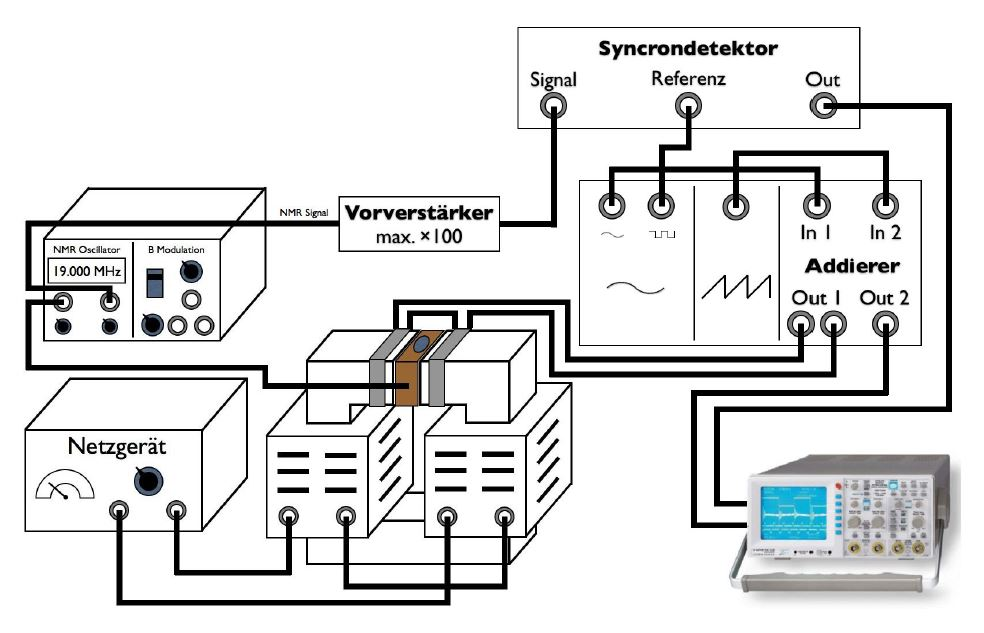
\includegraphics[scale=0.8]{Bild/Setup2}
=======
For the second part the lock-in method is used since it is more precise duo to its lower background noise. Instead of the former absorption curve this method gives the differentiated curve. For the modulation of the magnetic field the superposition of a sine and a sawtooth is used. Here the sawtooth is used mainly for the variance of the field while the sine is used to create the differentiated signal since it has a similar frequency to the reference signal. The former minima of the absorption curve will now be the 'Nulldurchgang' of the signal. The moment the 'Nulldurchgang' of both measured signals overlap the correct resonance frequency is hit. Examples of both signals are shown in figure \ref{SägezahnBsp} and the setup is given in figure \ref{Exp_part2}.
\begin{figure}[h]
	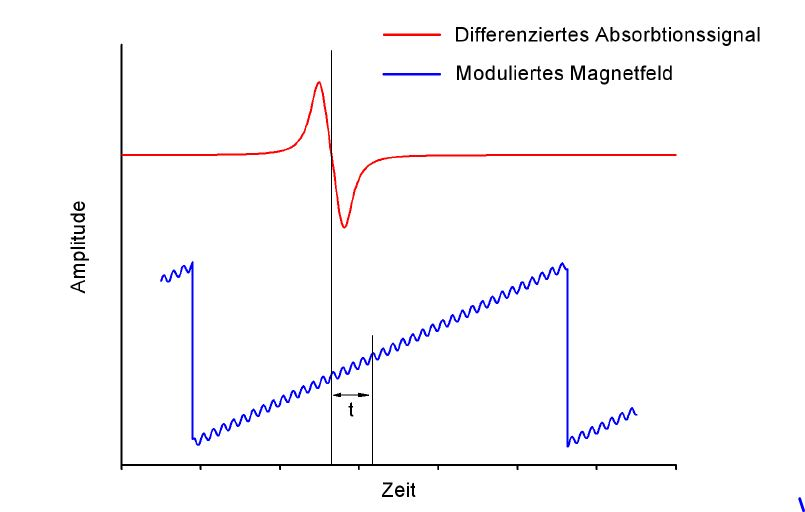
\includegraphics[scale=1]{Bild/BspLockIn}
	\centering
	\caption{Derived absorption signal in red. Superposition of sine and sawtooth waves with both 'Nulldurchgängen' aligned.}
	\label{SägezahnBsp}
\end{figure}
\begin{figure}[h]
	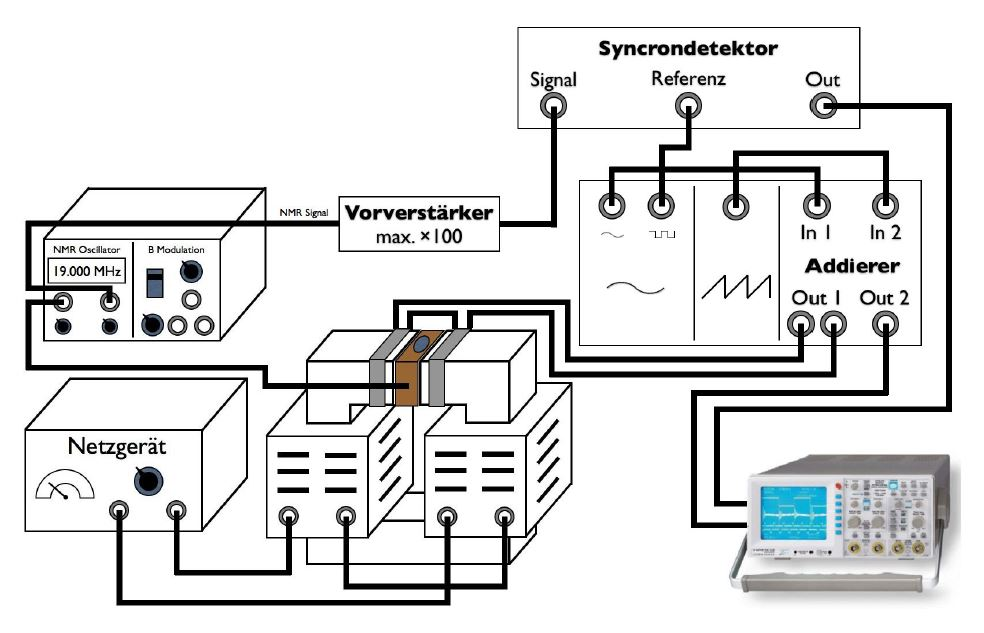
\includegraphics[scale=1]{Bild/Setup2}
>>>>>>> 1d836431a04c9587bc1733433202db64440414f4
	\centering
	\caption[Block Diagram for Setup 2]{Setup for measuring the resonance frequency with the lock-in method.}
	\label{Exp_part2}
\end{figure}

